\documentclass[titlepage]{article}
\usepackage[utf8]{inputenc}
%%%%%%%%%%%%%%%%%%%%%%%%%%%%%%%%%%%%%%%%%%%%
% ------ Packages ------
\usepackage{fullpage}           %sets margins to 1"
\usepackage{titling}
\usepackage[none]{hyphenat}     %NO HYPHENS
\usepackage[toc,page]{appendix}

\usepackage{tikz}               %graphics
\usepackage{framed}             %boxes in figures
\usepackage{multicol}           %columns
\usepackage{hyperref}           %links
\usepackage{amsmath,amstext}    %math
\usepackage{amsfonts}           %math fonts
\usepackage{mathtools}
% \usepackage{minted}             %code
\usepackage[parfill]{parskip}   %lineskip instead of indent
% \usepackage{gensymb}

\usepackage{caption}
\usepackage{subcaption}

\DeclarePairedDelimiter\ceil{\lceil}{\rceil}
\DeclarePairedDelimiter\floor{\lfloor}{\rfloor}

%%%%%%%%%%%%%%%%%%%%%%%%%%%%%%%%%%%%%%%%%%%%

%%%%%%%%%%%%%%%%%%%%%%%%%%%%%%%%%%%%%%%%%%%%
% ------ Package Preferences ------
\setlength{\droptitle}{-2cm}

\graphicspath{ {img/} }

% \hypersetup{                %color of links
%     colorlinks,
%     linkcolor=red,
%     urlcolor=blue
% }

\def\UrlBreaks{\do\/\do-} %url line breaks
%%%%%%%%%%%%%%%%%%%%%%%%%%%%%%%%%%%%%%%%%%%%

%%%%%%%%%%%%%%%%%%%%%%%%%%%%%%%%%%%%%%%%%%%%
% ------   Macros   ------
\renewcommand{\thesubsection}{\thesection.\alph{subsection}} %subsections to letters
\renewcommand{\thesubsubsection}{\thesubsection.\roman{subsubsection}}
\renewcommand{\baselinestretch}{1.25}

\newcommand{\dline}{\hrule \vskip -.2em \hrule} % double line

%%%%%%%%%%%%%%%%%%%%%%%%%%%%%%%%%%%%%%%%%%%%

%%%%%%%%%%%%%%%%%%%%%%%%%%%%%%%%%%%%%%%%%%%%
% ------ Title Block ------
\title{A review of modern bone trauma analysis\\ \large Forensic Anthropology, Wellesley College}
\author{Sophia Li}
\date{\today \\ \vspace{5em}}

%%%%%%%%%%%%%%%%%%%%%%%%%%%%%%%%%%%%%%%%%%%%


\begin{document}

% ------ Pre-Content ------
\maketitle

% ------   Content   ------

\section{Introduction}
This review paper aims to be a comprehensive summary of modern bone trauma analysis. It will begin with a section detailing bone physiology and bio-mechanics, specifically regarding changes to the material properties of the bone as the body decomposes. Additionally, it will summarize methods of determining ante-mortem trauma on the bone to peri/post-mortem trauma by examining the healing exhibited at the trauma site.

Additionally, as the approach to an investigation based on the type of trauma differs depending on the type of trauma observed on the bone, this paper will give a summary of current methods of identification and investigation for the five major types of bone trauma. These include ballistic, blast, blunt force, sharp force, and thermal trauma. Each section will begin with a description on the characteristics of the trauma, and methods of identification. It will follow with an overview of the current methods used in the medico-legal system to identify the tool used and the nature of the trauma event based on evidence found in the bone.

This paper will conclude with a discussion on the future of bone trauma analysis, and why trauma analysis is important to forensic anthropologists in the field today.

\section{Material properties of bone}
The human skeleton is the constantly changing frame of the body, with cell turnover ensuring that the bone will be able to grow, heal, and adapt. There are two main types of bone tissue, specifically cortical and cancellous(trabecular) bone. Cortical bone forms the hard hollow cylinder of the bone and is responsible for mechanical stability. Cancellous bone is the spongy interior of the cylinder, and is responsible for nutrient storage and transport. The tissues are biologically identical, but differences in the arrangement of the microstructure results in different material properties. Cortical bone forms about 80\% of the mass of the skeleton, and forms a hollow cynlinder within which the spongy cancellous bone resides.\cite{bone} Fig.\ref{fig:bone_struct} provides a cross-sectional view of the two types of ossesous tissue in an adult femur and provides numerical stress thresholds for adult bone.\\

\begin{figure}[h!]
\centering
\begin{subfigure}{.5\textwidth}
  \centering
  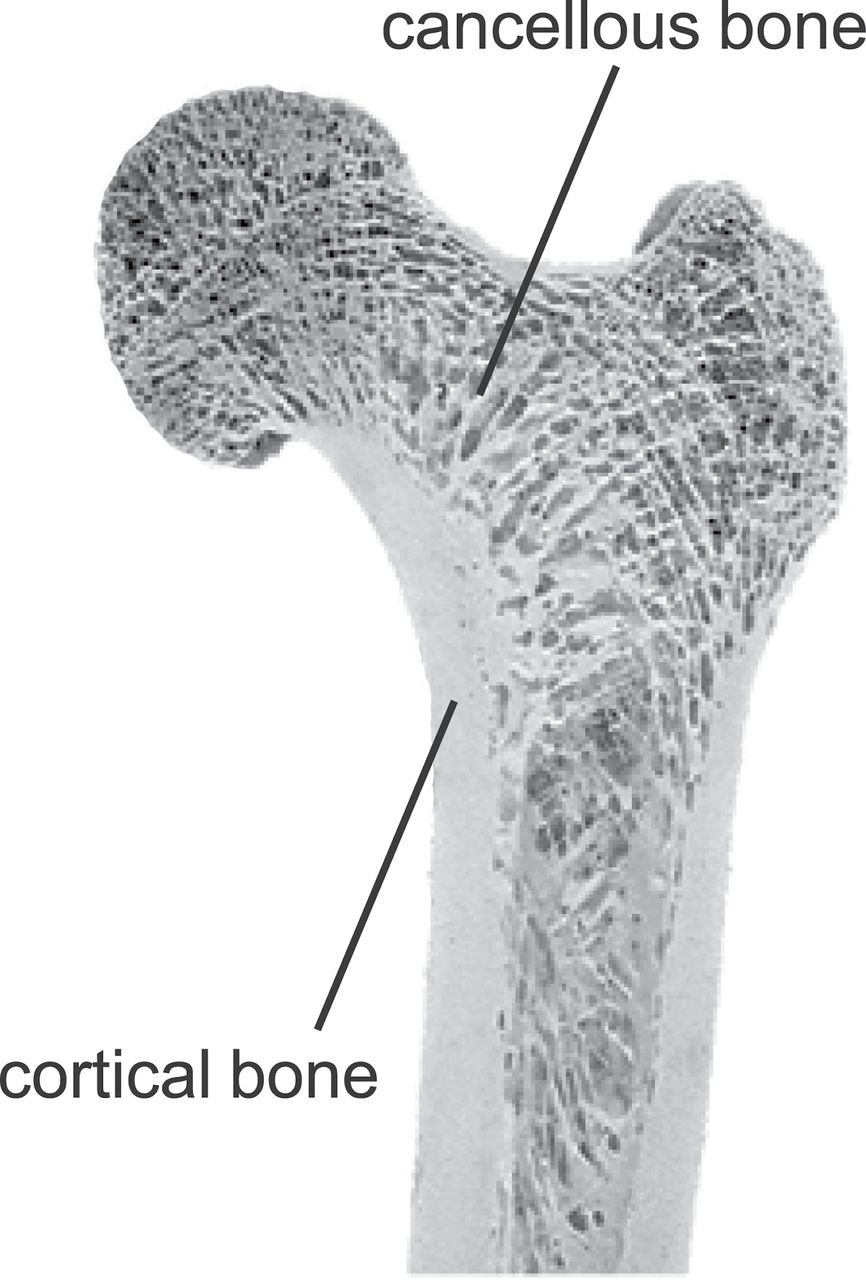
\includegraphics[width=.4\linewidth]{bone_microstructure}
  \caption{Adapted from \cite{cross-section}}
  \end{subfigure}%
\begin{subfigure}{.5\textwidth}
  \centering
  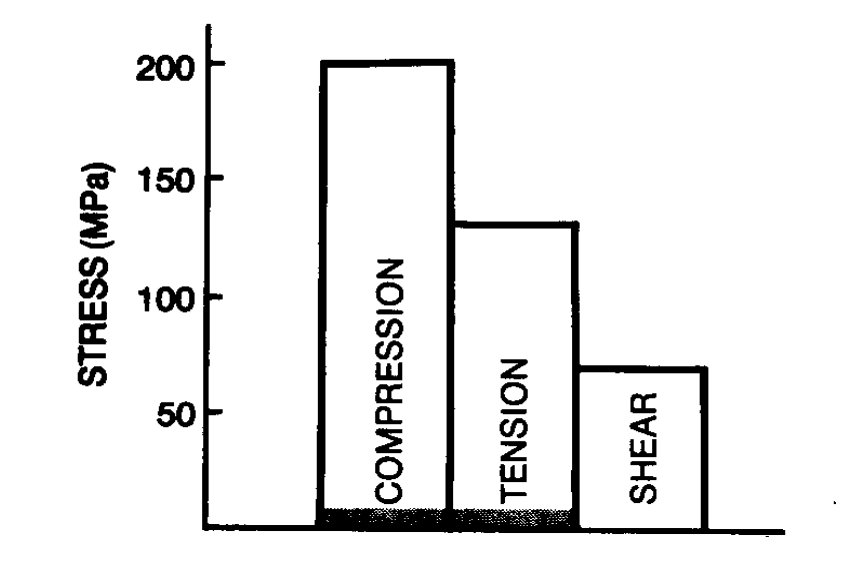
\includegraphics[width=.9\linewidth]{bone_stress}
  \caption{Adapted from \cite{stress}}
\end{subfigure}
\caption{(a) is a cross-section of a human femur, showing the difference between cancellous and cortical bone. (b) charts ultimate stress thresholds for adult cortical bone. Shaded areas indicate thresholds for cancellous bone.}
\label{fig:bone_struct}
\end{figure}

As can be seem from Fig.\ref{fig:bone_struct}.b, there are marked differences in strength between cortical and cancellous bone, thus the ratio of of the two at a trauma site will affect the definition of the mark left behind.  From Fig.\ref{fig:bone_struct}.a, it is observed that bone is strong against compressive and tensive forces, but weak against shear. This is consistent with typical loading forces bone experiences in day to day life. However, the bio-mechanics of a specific sample of bone will depend on the sampled individual. Factors like age, sex, location in body, and amount of water present will heavily affect the mechanical properties of the bone. Thus, any observations should take the unique context of the individual and the environment into account when characterizing marks left on bone material. Additionally, Fig.\ref{fig:bone_struct}.b notes that there are marked differences in strength between cortical and cancellous bone, thus the ratio of of the two at a trauma site will affect the definition of the mark left behind. Forensic investigators interested in timing fractures or marks observed on the bone should observe the following characteristics.

\textbf{Ante-mortem trauma}: Refers to trauma on the skeleton that occurs prior to the death of the individual. In-vivo bone exhibits healing, and edges of a fracture will be fairly smooth. If the trauma occured while the individual was young, there may be almost no signs of trauma happening at all. Some examples of ante-mortem trauma include lesions on the bone due to responses to infection, degenerative joint disease, or sugically implanted instruments. As healing rates differ depending on the characteristics of the individual, the same injury may look different from case to case.

\textbf{Peri-mortem trauma}: Refers to trauma occuring around death. Fracture patterns observed in peri-mortem trauma can be similar to those seen in ante-mortem trauma, but have sharper edges since no healing will have occured (in most cases). Patterns will show evidence of some terminal event, i.e fast collision with an object, but fracture edges will show characteristics of plastic deformation as the external fibers of the bone tissue begin to show micro-tears.

\textbf{Post-mortem damage}: Refers to damage occuring after death. Bone becomes brittle once it has dried out, and exhibits ceramic-like material properties. Fractures will be jagged and exhibit no healing, and discoloration of the bone may be observed in the case where damage exposes new surfaces of the bone after some time. Fracture patterns may also be irregular, and lack a common correlation to an event that caused the damage, i.e fractures resulting from post-mortem bone shrinkage.\cite{trauma, evid}

\begin{figure}[h!]
\centering
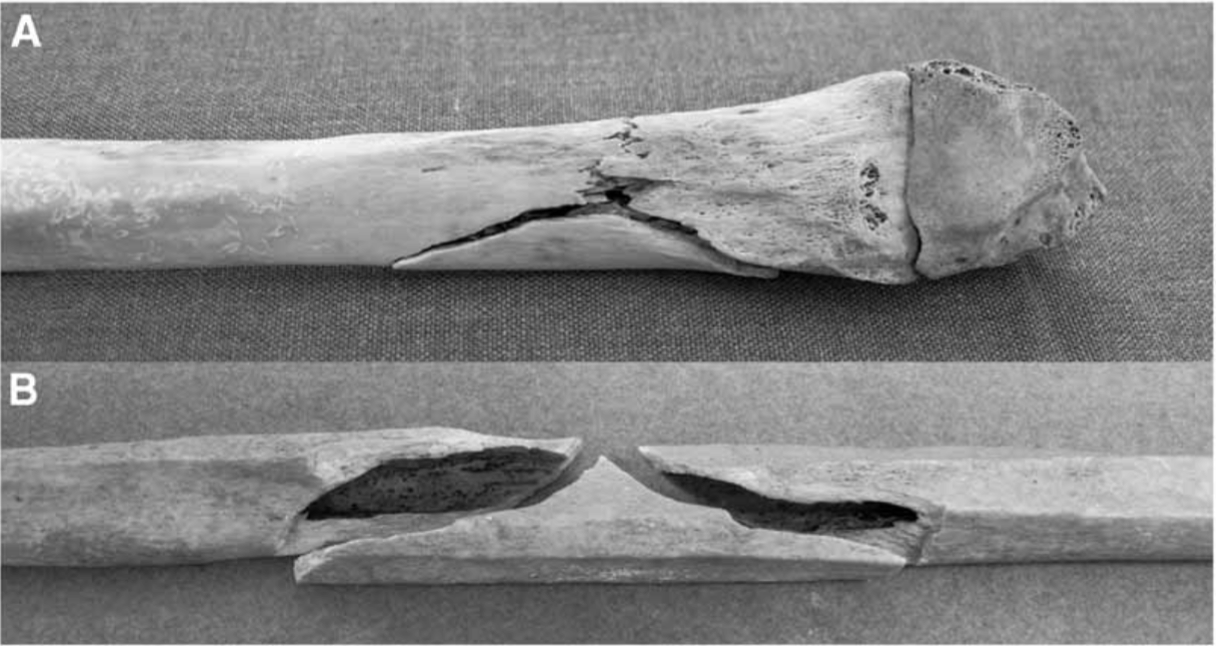
\includegraphics[width=.7\linewidth]{fracture}
\caption{Adapted from \cite{blunt-trauma}. Butterfly fracture on peri-mortem (A) and post-mortem (B) fibula. Note how there is delamination and evidence of plastic deformation on the peri-mortem fracture, but none of the sort on the post-mortem bone.}
\label{fig:fracture}
\end{figure}

Regardless of which kind of traumatic event has occured on the bone, the mechanics of the material remains constant. Due to inhomogenous composition of bone, it is difficult to exactly predict the fracture response of bone to a stimulus. A study conducted by Ramana Sadananda concludes that a probabilistic approach using Weibull statistics was significantly accurate in predicting fracture probability of three types of chicken bones.\cite{fracture-analysis} Though the study was not conducted on human bones, it still shows that the Weibull distribution is applicable in quantitatively determining the material strength of bone. The same kind of statistics are used for failure analysis in many engineering fields, indicating that there may be an overlap of knowledge that anthropologists may draw from. As the bio-mechanical properties of bone dictate the response of bone to trauma, being able to simulate and predict fractures provides important information to a forensic anthropologist.

\section{Ballistic}
Ballistic trauma on bone is usually the result of a bullet or an explosive, though this categorization may be applied to any fast traveling object that has collided with bone. Features that indicate possible ballistic trauma include the presence of a projectile that can be associated with bone, fracture patterns corresponding to a high velocity impact, or fragmentary foreign material found within the bone or the environment.\cite{trauma}

Entrance wounds are typically smaller than exit wounds, due to bullets entering the body at a higher speed than when exiting. A projectile may plastically deform or shatter as it travels through the body, leaving fragmentary material embedded in soft tissue along its track. If the projectile results in a penetrating wound, it will enter the body but not exit. A straight line path between an entrace and exit wound does not ensure the two are connected, as the projectile may travel in a manner of ways as it interacts with other tissues in the body.\cite{ballistic-trauma} If an exit wound is present, then the projectile is perforating. Exit wounds are typically larger and result in more fragmentary material because the bullet hits the bone with less force, and thus has a longer amount of time to transfer energy to the bone before crossing the fracture threshold of the bone and passing through. This energy transfer results in typically larger fractures. A third type of ballistic trauma occurs when the projectile shatters while within the body, creating secondary exit wounds as the fragments exit the body. Thus, while there will always be an entrace wound, the presence or the number of exit wounds depends on the situation.

Fig.\ref{fig:gunshot}.a is an example of a penetrating wound. The entrace wound (denoted by the solid arrow) shows the radially branching fractures from a small hole in the frontal bone. The exit wound is larger, with fragments of bone breaking from the skull.

\begin{figure}[h!]
\centering
\begin{subfigure}{.5\textwidth}
  \centering
  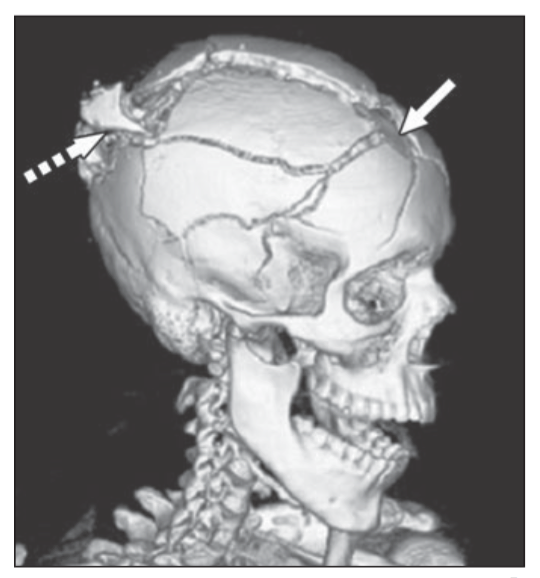
\includegraphics[width=.7\linewidth]{gunshot1}
  \end{subfigure}%
\begin{subfigure}{.5\textwidth}
  \centering
  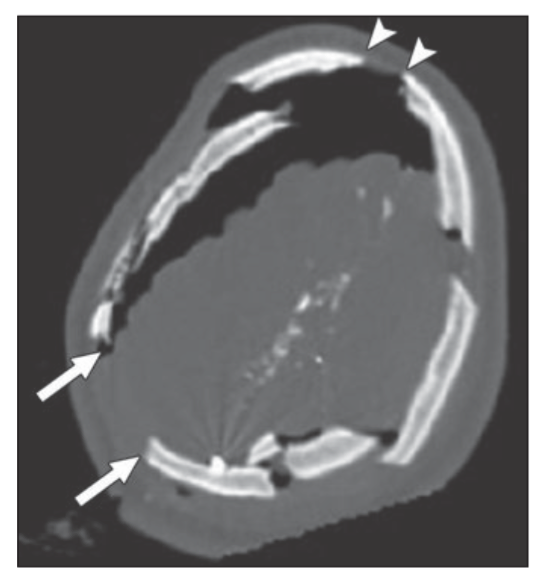
\includegraphics[width=.7\linewidth]{gunshot2}
\end{subfigure}
\caption{Adapted from \cite{ballistic-trauma}. (a) is a 3D reconstruction image, where the solid arrow indicates the entrance and the dotted arrow indicates the exit wound. (b) is a CT scan, where the arrows indicate entrance while the arrowheads indicate exit wound.}
\label{fig:gunshot}
\end{figure}

Additionally, beveling on the wound will indicate the direction of travel. Fig.\ref{fig:gunshot}.b shows the differences in beveling between entrance and exit wounds. Beveling points towards the internal of the skull for the entrance wound, while the opposite is true for the exit wound.\cite{ballistic-trauma}

Imaging technology is useful in documenting the exact state of the bone, and digitizing information is an additional safeguard in preventing evidence from being misplaced. In investigating ballistic trauma, computer tomography (CT) and magnetic resonance imaging (MRI) have been helpful in identifying potential entrance and exit wounds, and the path of a projectile through the body. Fig.\ref{fig:entrance_wound} and Fig.\ref{fig:exit_wound} are examples of how faithfully CT scans can reproduce the physical model.

\begin{figure}[h!]
\centering
\begin{subfigure}{.5\textwidth}
  \centering
  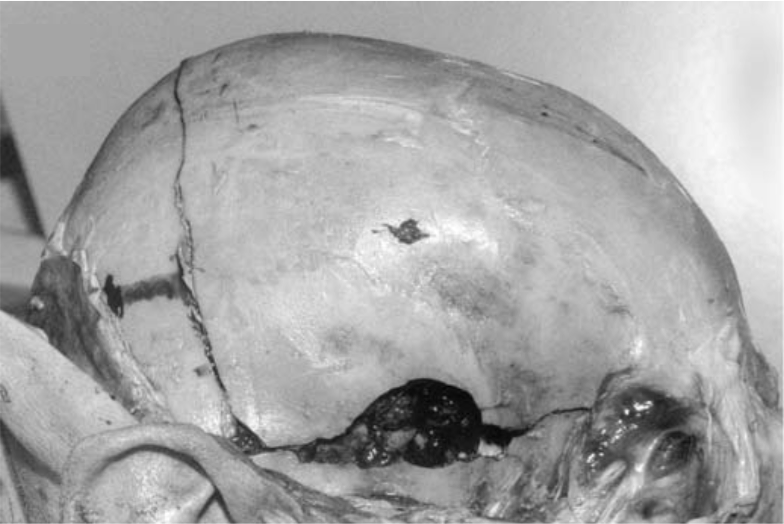
\includegraphics[width=.7\linewidth]{entrance}
  \end{subfigure}%
\begin{subfigure}{.5\textwidth}
  \centering
  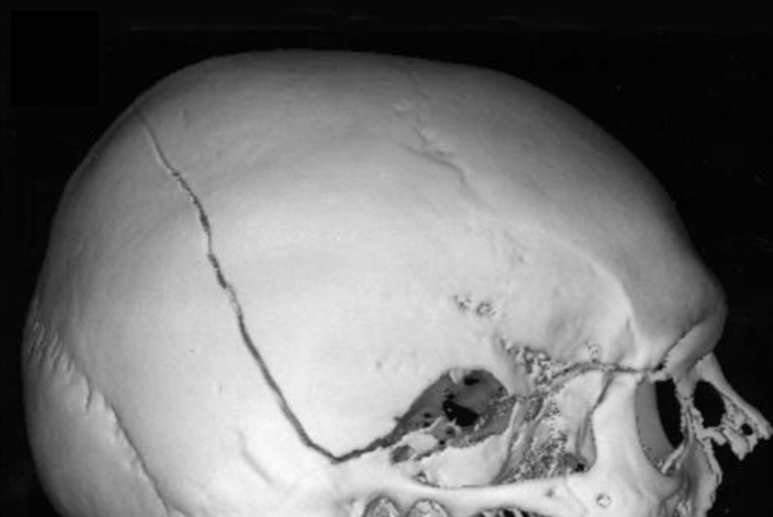
\includegraphics[width=.7\linewidth]{entrance_ct}
\end{subfigure}
\caption{Adapted from \cite{post-imaging}. (a) is a photo of a bullet entrance wound, (b) is a 3D CT reconstruction}
\label{fig:entrance_wound}
\end{figure}

\begin{figure}[h!]
\centering
\begin{subfigure}{.5\textwidth}
  \centering
  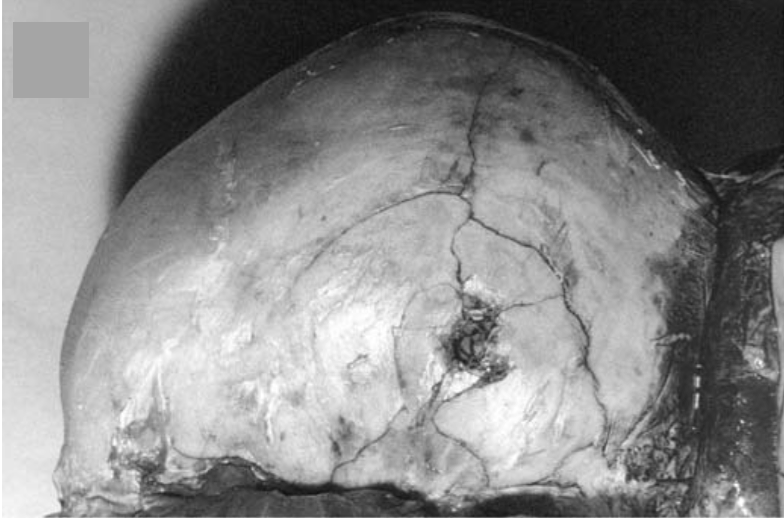
\includegraphics[width=.7\linewidth]{exit}
  \end{subfigure}%
\begin{subfigure}{.5\textwidth}
  \centering
  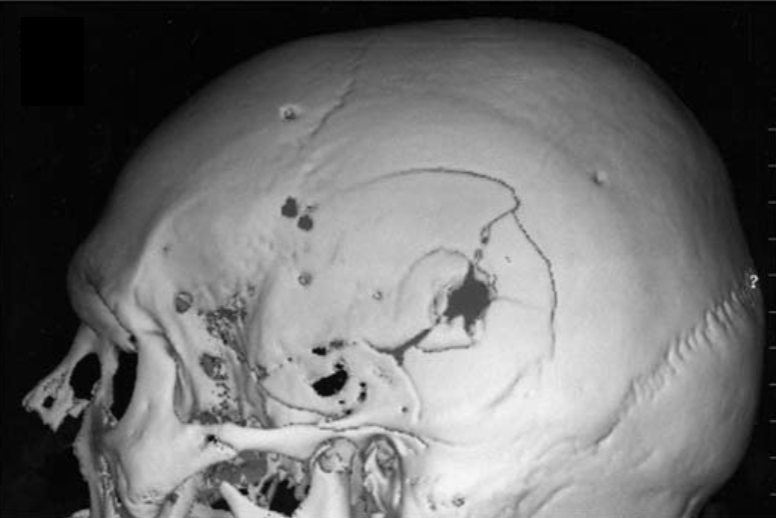
\includegraphics[width=.7\linewidth]{exit_ct}
\end{subfigure}
\caption{Adapted from \cite{post-imaging}. (a) is a photo of a bullet exit wound, (b) is a 3D CT reconstruction}
\label{fig:exit_wound}
\end{figure}

While hard tissue is good at providing investigators with information about the entrance and exit of a bullet, it is not quite as informative in recording the path of the bullet through the body. However, CT imaging works well on both soft and hard tissue and can preserve a cadavar from further decay by recording its current state into a digital form. This quality is especially important for ballistic trauma, as the path of the projectile can be inferred from the CT scan by revealing lanes of tissue damage through the body and identification of possible projectile fragments embedded in soft tissue.

\section{Blunt force trauma}
While ballistic trauma can be classified as blunt force trauma, in the context of this paper blunt force trauma will refer to trauma resulting from a low velocity impact from a blunt object or blunt surface. Features suggesting blunt force trauma include plastic deformation, delamination, tool marks/impressions at trauma site, or fracture patterns on the bone suggesting low velocity impact.\cite{trauma}

During low velocity impact, the bone will have more time to bend and deform in response to the stress before it fails. A study by Kulin\cite{post-imaging} tested equine bones at different strain rates. They found that the slower the strain rate, the more fragmentation occured in the microstructure of the bone. As bone is viscoelastic, a slower strain rate gives the bone time to go through plastic deformation before failure. Fractures from slow loading rates were jagged and propagated away from the main crack path, limiting the overall fracture length as energy was dissapated over a greater surface area of bone. Under faster loading conditions, the fractures were straighter and had less perhipheral damage. This study showed that fracture propagation was dependant on the rate of the loading force. Since blunt force trauma is the result of a slow loading force, fractures resulting from it will typically propagate like a web across the surface area of bone instead of forming one major crack as the cracks travel around embedded vascular structures in the bone. Fig.\ref{fig:skull} demonstrates the characteristic propagation of fractures from the main blunt force trauma impact site.

\begin{figure}[h!]
\centering
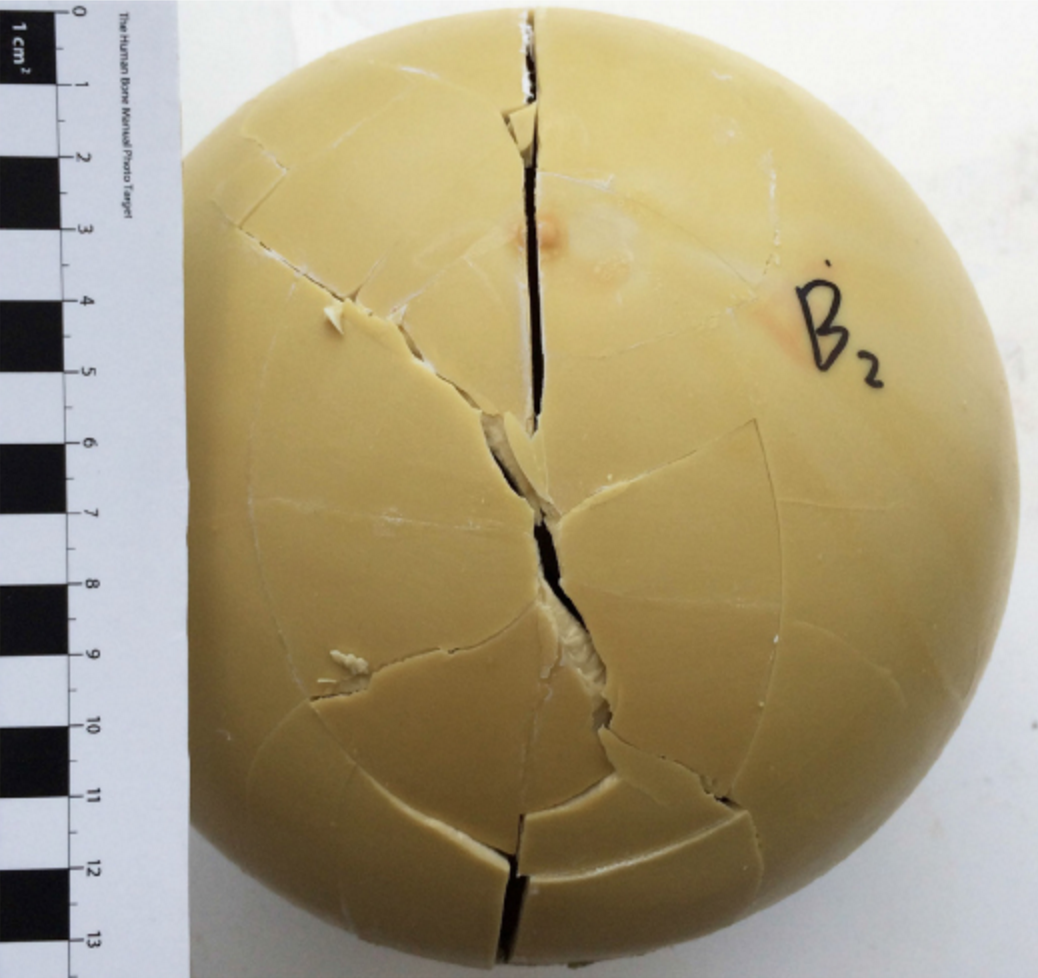
\includegraphics[width=.4\linewidth]{blunt_trauma}
\caption{Adapted from \cite{craniums}. Depressed fracture on sphere simulating a free-moving head after strike with a baseball bat}
\label{fig:skull}
\end{figure}

Different kinds of applied force will exhibit itself characteristic fracture patterns as well. Knowledge of these patterns can provide additional information about the events leading up to the fracture.

\begin{figure}[h!]
\centering
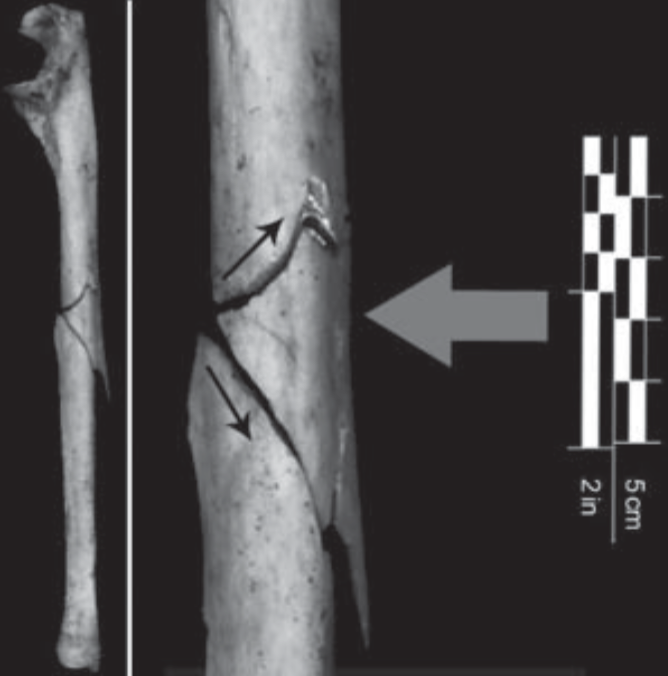
\includegraphics[width=.4\linewidth]{butterfly}
\caption{Adapted from \cite{bft}. Butterfly fracture on ulna, the white arrow indicates the direction of impact. The bone fails at the body of the butterly, fracturing upwards along the black arrow}
\label{fig:butterfly-fracture}
\end{figure}

Fig.\ref{fig:butterfly-fracture} is a butterfly fracture on the ulna. Due to the organization of the osseous fibers, fractures will tend to propagate down the length of the bone.\cite{mechanics} As observed in Fig.\ref{fig:butterfly-fracture}, the bone fails and cracks propagate diagonally. Since fractures are always the result of interactions between forces and the morphology of the bone, the presence of a butterfly fracture on a long bone immediately provides evidence of an impact perpendicular to the length of the bone. As such, it becomes valuable to have a fully modeled human skeleton so that anthopologists will have immediate predictions as to forces necessary to produce fracture patterns. Computational human skeleon models are not robust enough to act as a substitute to real bone, though the area is very much in active research. Researchers have also experimented with nonhuman animal models, mostly focusing with porcine and deer due to similarities with the human skeleton. Current tests conducted these animals have provided information about how weathering effects evidence of blunt force trauma, showing it is possible for bone to retain characteristics of trauma even after 52 weeks of exposure and freeze-thaw cycles.\cite{bft}

\newpage
\section{Sharp force trauma}
Sharp force trauma is characterized by trauma resulting from a tool that is edged, pointed, or beveled. Features indicating this kind of trauma include straight-lined incisions, punctures or gouges, clefs or kerfs. Considerations must be taken when examining the wound, since alterations to the bone like scrapes or score marks are not classified as sharp force trauma. \cite{trauma}

When examining bones with evidence of sharp force trauma, Casting is an immediately viable option, and is a non-destructive way of providing investigators a method of examining the wound. However, casting on on soft-tissue has been met with mixed success, and is unable to provide information to investigators on the micro scale about the incision. However, it is possible to estimate the motion of the tool based on whether it is a slash (the incision is wider than it is deep), or a stab (the incision is deeper than it is wide) through visual inspection. \cite{serrated} Macro inspection of the wound at a visual scale can qualitatively describe the tool used in the trauma down to a class, such as "single edged" or "beveled". The handedness of an attacker, or whether a wound is self inflicted can be determined by the angle of the incision in context to the position of the body.

Crack propagation happens more readily in the lateral direction due to the organization of the bone tissue fibers.\cite{mechanics} In cases where the bone has experianced sharp force trauma,


Micro-CT scanning technology is used to give greater insight to the patterned marks left within bone from sharp force trauma, by giving investigators cross-sectional view of the impact site. Tests conducted via sharp force inpact analyzed by micro-CT scanning were able to correctly determine the size and shape of a knife, in addition to the angle of impact in most cases. The tests were not quite as accurate when the knife was excessively rocked or rotated within the bone, though examining the wound profile and the tip of the knife allows better precision.\cite{micro-ct}


\newpage
\section{Thermal trauma}
Thermal trauma is the result of bone that is in direct contact with high temperatures for a significant amount of time. Characterics of bone with thermal trauma include shrinkage, discoloration, calcification, or an observable burn pattern on the surface of the bone.\cite{trauma}

Bone that has undergone thermal trauma is typically in a fragmentary state, making retreival difficult. Establishing a minimum number of individuals is hard as well, thanks to possible comingling that may occur at the location of the fire. Bones exposed to high temperatures will shrink due to the rapid evaporation of water, though the amount of shrinking will depend on a variety of internal (age, sex, height) and external (fire temperature, oxygen content) factors.  Shrinkage begins at temperatures of 700C, with augmented degrees of shrinkage until 800C when no more shrinkage occurs. Bone also undergoes structural changes during the temperature ramp, with organic material like cellulose being destroyed at 400C, recrystallization of the bone mineral at 600C, and melting of bone mineral at 1600C. \cite{fire}

In the case where a fire is set in an attempt to hide a homicide, analysis of possible peri-mortem trauma that is unrelated to the fire is important in providing factual evidence on the case. Heat-induced fractures have an irregular pattern when compared to those seen in impact based trauma. Curved transverse fractures occuring in a stacked arc formation across the grain of the bone are most commonly associated with the reduction of soft tissue during a fire. Delamination, described as the peeling or flaking of the bone's outer layers, occurs due to the separation of cortical and cancellous bone. A cracked and dehydrated appearance of the outer layers of cortical bone is also typical due to the rapid dehydration of the bone during a fire.\cite{fire-bone}

Conversely, fractures due to impact-based trauma should obey bone bio-mechanics. Clean, long fractures are indicative of some high energy low duration impact, while shallow jagged fractures imply the a low energy high duration impact. Even after bone is burned, these features still remain.

\begin{figure}[h!]
\centering
\begin{subfigure}{.5\textwidth}
  \centering
  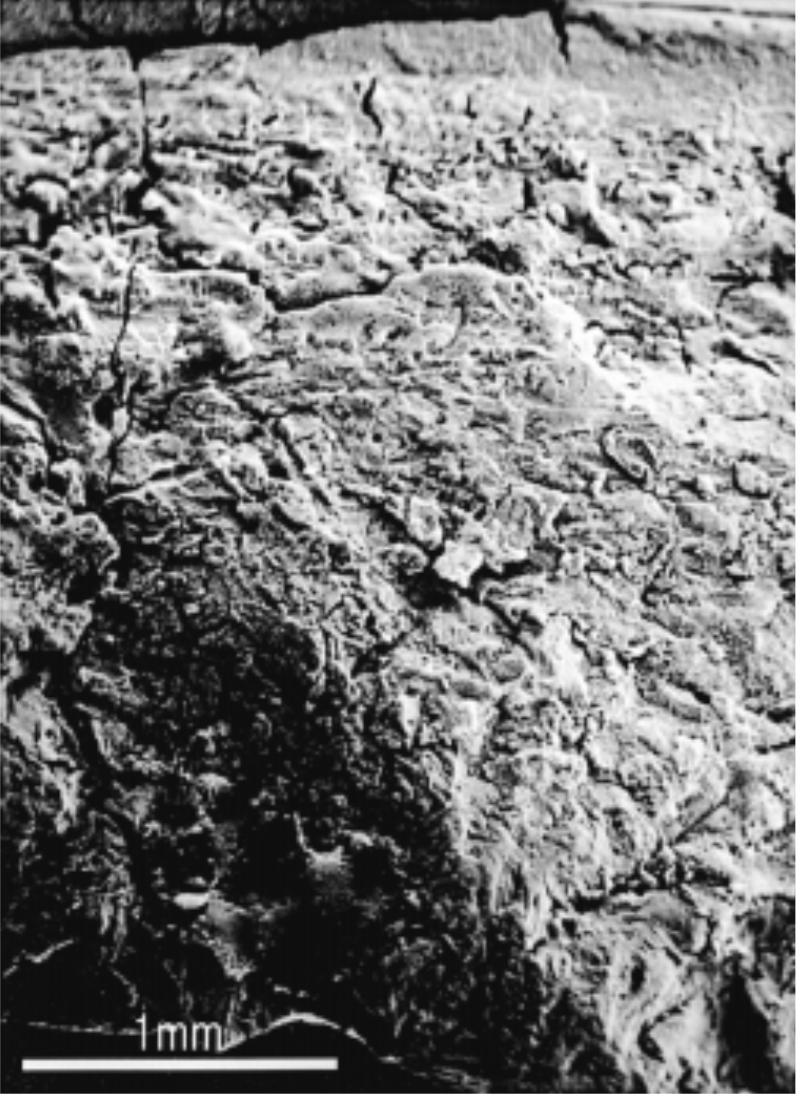
\includegraphics[width=.7\linewidth]{trauma_transverse}
  \end{subfigure}%
\begin{subfigure}{.5\textwidth}
  \centering
  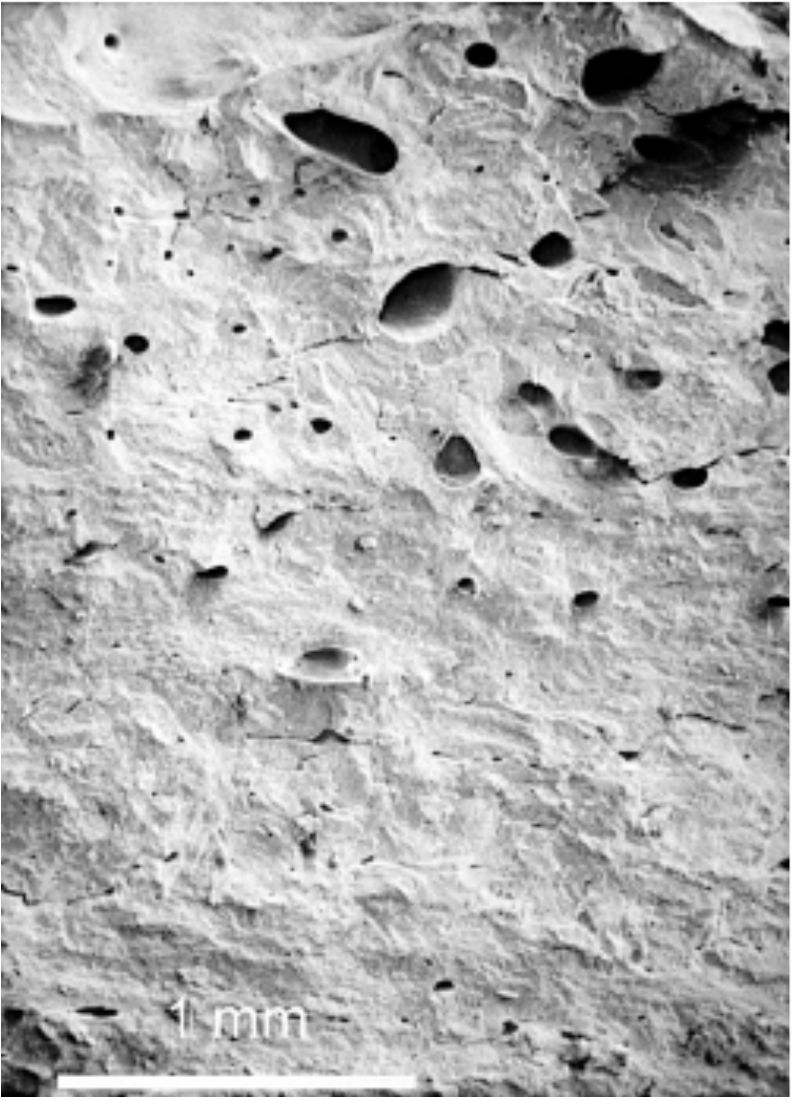
\includegraphics[width=.7\linewidth]{heat_transverse}
\end{subfigure}
\caption{Adapted from \cite{fire-bone}. Images of transverse fractures on burned porcine femur. (a) is a photo of a trauma induced transverse fracture. (b) is a heat induced transverse fracture.}
\label{fig:fracture_comp}
\end{figure}

Fig.\ref{fig:fracture_comp} shows the differences between fractures induced by heat and fractures from impact based trauma. When viewed at 30x magnification, the surface of the fracture is quite different between the two. Fig.\ref{fig:fracture_comp}.b shows that the fracture surface of a heat induced fracture is quite clean, and is very smooth when compared to the impact trauma induced fracture in Fig.\ref{fig:fracture_comp}.a. Since recrystallization of bone mineral occurs at 600C, clean fractures like these indicate that the fractures occured late in the burning process or after the bone has cooled.

\begin{figure}[h!]
\centering
\begin{subfigure}{.5\textwidth}
  \centering
  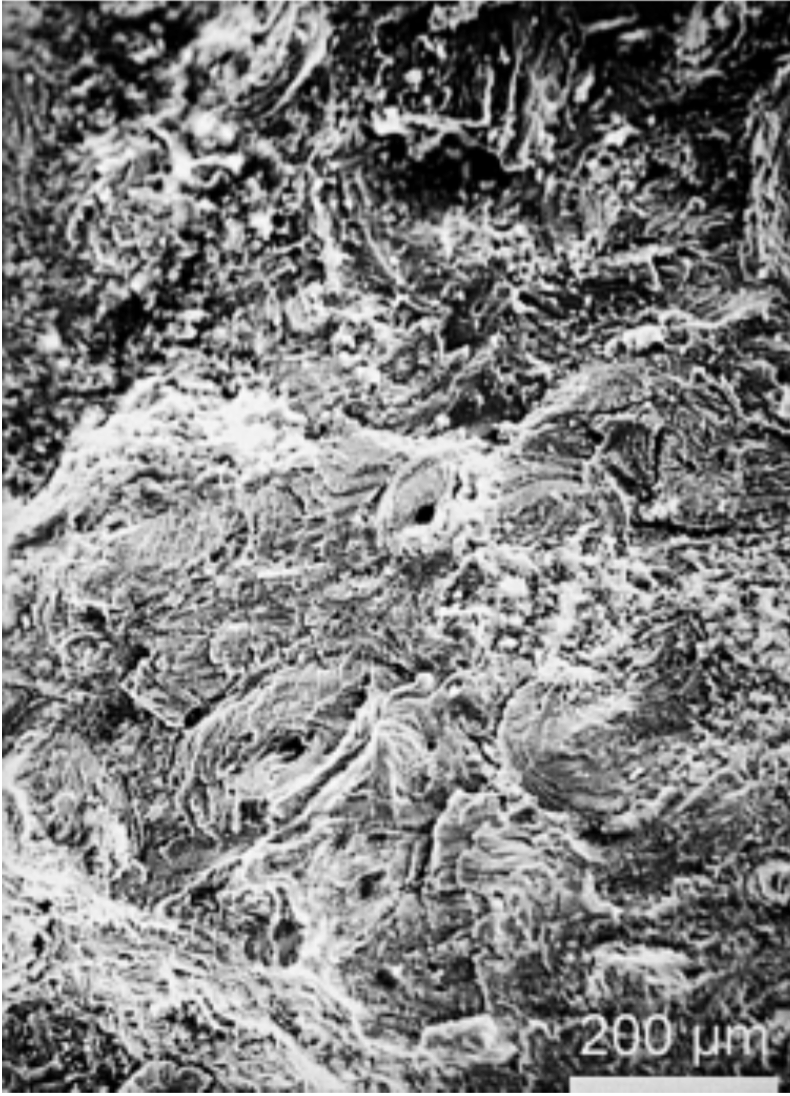
\includegraphics[width=.7\linewidth]{unburned_transverse}
  \end{subfigure}%
\begin{subfigure}{.5\textwidth}
  \centering
  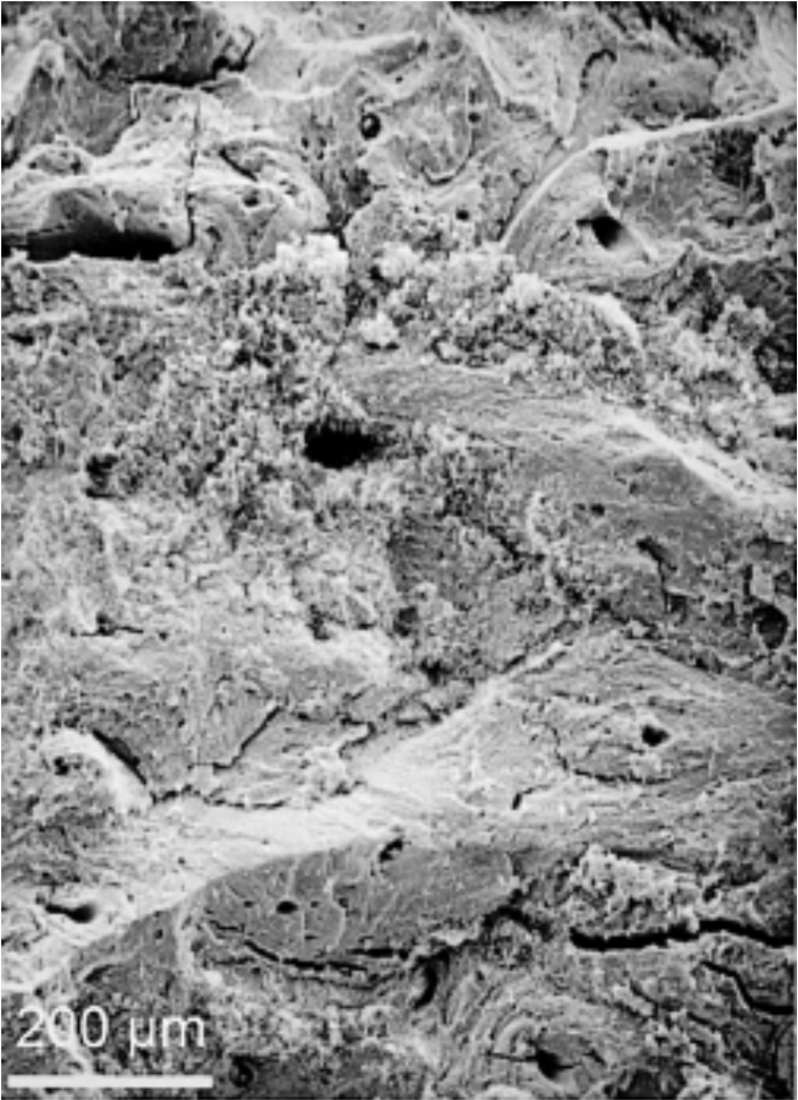
\includegraphics[width=.7\linewidth]{burned_transverse}
\end{subfigure}
\caption{Adapted from \cite{fire-bone}. (a) is a photo of a unburned transverse fracture on a porcine femur. (b) is an burned version of the same.}
\label{fig:burn_fracture}
\end{figure}

Fig.\ref{fig:burn_fracture} is a 100x magnification of a transverse fracture on a porcine femur via scanning electron microscope. Fig.\ref{fig:burn_fracture}.a shows an unburned fracture, where the definition of the fracture surface is greater than that of the burned version shown in Fig.\ref{fig:burn_fracture}.b. As already observed in Fig.\ref{fig:fracture_comp}, fires will erase definition due to high temperatures causing changes to the structure of the boney material. Sediment like soot or ash will also settle inside fractures, potentially causing issues when attempting to observe detail of fracture sites.

A study by Herrman concluded that even with simple optical microscope analysis, it was possible to identify post-mortem sharp force trauma following incineration of bone as the evidence left on bone is distinctive enough to be recognizable even after fragmentation has occured. Fractures resulting from blunt force or ballistic trauma required rigorous examination at high magnifications (100x) because the resulting fractures were quite similar to changes that may occur to bone during exposure to high temperatures. However, they concluded that large fragmentary bone material were more likely to be due to post-mortem trauma, while small fragments were more likely to be due to flaking of the bone from the fire. \cite{fire-bone}

\newpage
\section{Conclusion}

When observing fatal cranial fractures due to blunt force trauma, it is found that linear fractures on the right site of the skull are common in falls while linear fractures on the left side are common in homicide cases. As the majority of people are right handed, most will attempt to catch a fall with their right hand which results in the right side of their head hitting the ground first. In cases of homicide, if the victim and assailant are facing each other, the left side of the skull is likely to show damage. If the assailant is behind the vicim, then the damage is still likely to appear on the right side.\cite{craniums}

\newpage
\bibliographystyle{ieeetr}   % this means that the order of references
			    % is dtermined by the order in which the
			    % \cite and \nocite commands appear
\bibliography{mybib.bib}

\end{document}
\end{document}
